% !TEX program = pdflatex
%% ---------------------------------------------------------------------------
%%  EEE F111 — Electrical Sciences   CORE MASTERY MAPS
%% ---------------------------------------------------------------------------
\documentclass[a4paper]{article}

%% --- Fonts -------------------------------------------------------------------
\usepackage[T1]{fontenc}
\usepackage{tgpagella}
\usepackage{tgheros}
\usepackage{mathpazo}

%% --- Layout ------------------------------------------------------------------
\usepackage[a4paper, landscape, margin=0.6cm]{geometry}

%% --- Colors ------------------------------------------------------------------
\usepackage{xcolor}
\definecolor{DeepNavy}{HTML}{0f172a}
\definecolor{ElectricBlue}{HTML}{2563eb}
\definecolor{SkyBlueBG}{HTML}{dbeafe}
\definecolor{Amber}{HTML}{d97706}
\definecolor{AmberBG}{HTML}{fef3c7}
\definecolor{Emerald}{HTML}{059669}
\definecolor{EmeraldBG}{HTML}{d1fae5}
\definecolor{SlateGray}{HTML}{64748b}
\definecolor{LightBG}{HTML}{f8fafc}
\definecolor{CardBorder}{HTML}{e2e8f0}
\definecolor{CoralRed}{HTML}{dc2626}
\definecolor{CoralBG}{HTML}{fee2e2}
\definecolor{Purple}{HTML}{7c3aed}
\definecolor{PurpleBG}{HTML}{ede9fe}
\definecolor{Teal}{HTML}{0d9488}
\definecolor{Crimson}{HTML}{be185d}
\definecolor{Indigo}{HTML}{4338ca}

%% --- TikZ --------------------------------------------------------------------
\usepackage{tikz}
\usetikzlibrary{mindmap, trees, backgrounds, calc, arrows.meta, positioning, shapes.geometric, fit, shadows.blur}

%% --- Misc --------------------------------------------------------------------
\usepackage{amsmath, amssymb}
\usepackage{fontawesome5}
\usepackage[hidelinks]{hyperref}
\pdfstringdefDisableCommands{}

\pagestyle{empty}
\setlength{\parskip}{0pt}
\setlength{\parindent}{0pt}

%% --- Shared Styles -----------------------------------------------------------
\tikzset{
  fcterm/.style={rectangle, rounded corners=12pt, draw=DeepNavy, fill=DeepNavy, text=white, text width=#1, align=center, font=\sffamily\small\bfseries, minimum height=0.85cm, inner sep=5pt, blur shadow={shadow blur steps=3}},
  fcterm/.default=4.2cm,
  fcproc/.style 2 args={rectangle, rounded corners=5pt, draw=#1, fill=#2, text width=4.2cm, align=center, font=\sffamily\footnotesize, minimum height=0.85cm, inner sep=5pt, blur shadow={shadow blur steps=1}},
  fcdec/.style={diamond, aspect=2.4, draw=Amber, fill=AmberBG, text width=3.2cm, align=center, font=\sffamily\footnotesize\bfseries, inner sep=2pt, blur shadow={shadow blur steps=1}},
  fcok/.style={rectangle, rounded corners=8pt, draw=#1!80!black, fill=#1, text=white, text width=3.0cm, align=center, font=\sffamily\small\bfseries, minimum height=0.85cm, inner sep=5pt, blur shadow={shadow blur steps=2}},
  fcok/.default=Emerald,
  fcwarn/.style={rectangle, rounded corners=5pt, draw=CoralRed, fill=CoralBG, text width=3.0cm, align=center, font=\sffamily\footnotesize, minimum height=0.8cm, inner sep=5pt, blur shadow={shadow blur steps=1}},
  fcarr/.style={->, >=Stealth, line width=1.2pt, draw=SlateGray},
  lyes/.style={font=\sffamily\scriptsize\bfseries, text=Emerald, fill=white, inner sep=1pt},
  lno/.style={font=\sffamily\scriptsize\bfseries, text=CoralRed, fill=white, inner sep=1pt},
  %% New grid box style
  cheatbox/.style={rectangle, rounded corners=8pt, draw=#1!80!black, fill=#1!5, line width=1.5pt, inner sep=8pt, text width=6.3cm, align=left, blur shadow={shadow blur steps=3}},
}

\newcommand{\cmhead}[3]{%
  \noindent\begin{tikzpicture}
    \fill[DeepNavy] (0,0) rectangle (\textwidth, 1.0cm);
    \fill[#1]       (0,-0.15cm) rectangle (\textwidth, -0.3cm);
    \node[anchor=west, text=white, font=\bfseries\sffamily\Large, inner xsep=12pt] at (0, 0.48cm)
      {\faMap\enspace EEE F111 Core Mastery\enspace \textcolor{#1!60!white}{|}\enspace #2};
    \node[anchor=east, text=LightBG, font=\small\sffamily\bfseries, inner xsep=12pt] at (\textwidth, 0.48cm) {#3};
  \end{tikzpicture}\par\vspace{10pt}}

\begin{document}

%% -----------------------------------------------------------------------------
%% PAGE 1 — MASTER CHEAT SHEET (Replaces empty Mind Map)
%% -----------------------------------------------------------------------------
\cmhead{ElectricBlue}{Master Formula \& Concept Dashboard}{Cheat Sheet Overview}

\vspace{0.1cm}
\begin{center}
\begin{tikzpicture}[node distance=0.3cm and 0.3cm]

  %% ROW 1
  \node[cheatbox=ElectricBlue] (box1) {
    \vspace{-0.3cm}
    \begin{flushleft}
    \textcolor{ElectricBlue}{\faProjectDiagram}\enspace \textbf{\large 1. DC Network Theorems}\\[4pt]
    {\footnotesize
    \textbf{Mesh (KVL):} Assign $i$ loops. Sum $V=0$.\\
    \textbf{Nodal (KCL):} Assign $V$ nodes. Sum leaving $I=0$.\\
    \textbf{Superposition:} Turn off independent sources $1$ by $1$ ($V\to$ short, $I\to$ open). Sum responses.\\[4pt]
    \textbf{Thévenin/Norton:}\\
    $V_{TH} = V_{oc}$ (open circuit voltage)\\
    $R_{TH} = R_{in}$ (dead sources)\\
    $I_N = V_{TH} / R_{TH}$\\[4pt]
    \textbf{Max Power Transfer:} $R_L = R_{TH}$\\
    $P_{max} = \frac{V_{TH}^2}{4R_{TH}}$
    }
    \end{flushleft}
  };

  \node[cheatbox=Teal, right=of box1] (box2) {
    \vspace{-0.3cm}
    \begin{flushleft}
    \textcolor{Teal}{\faBolt}\enspace \textbf{\large 2. AC Circuits \& Power}\\[4pt]
    {\footnotesize
    \textbf{Impedance:} $Z_R=R$, $Z_L=j\omega L$, $Z_C=\frac{1}{j\omega C}$\\
    \textbf{Complex Power:} $\mathbf{S} = \mathbf{V}_\text{rms} \mathbf{I}_\text{rms}^* = P + jQ$\\[4pt]
    \textbf{Real Power (P):} $V_{rms} I_{rms} \cos\theta$ (W)\\
    \textbf{Reactive (Q):} $V_{rms} I_{rms} \sin\theta$ (VAR)\\
    \textbf{Apparent (|S|):} $\sqrt{P^2+Q^2}$ (VA)\\[4pt]
    \textbf{Power Factor:} $pf = \cos(\theta_v - \theta_i) = P / |S|$\\[4pt]
    \textbf{Resonance:} Reactances cancel ($X_L = X_C$).\\ $\omega_0 = \frac{1}{\sqrt{LC}}$
    }
    \end{flushleft}
  };

  \node[cheatbox=Crimson, right=of box2] (box3) {
    \vspace{-0.3cm}
    \begin{flushleft}
    \textcolor{Crimson}{\faLayerGroup}\enspace \textbf{\large 3. Three-Phase Systems}\\[4pt]
    {\footnotesize
    \textbf{Star (Y) Connection:}\\
    $V_L = \sqrt{3} V_{ph} \angle 30^\circ$\\
    $I_L = I_{ph}$\\[4pt]
    \textbf{Delta ($\Delta$) Connection:}\\
    $V_L = V_{ph}$\\
    $I_L = \sqrt{3} I_{ph} \angle -30^\circ$\\[4pt]
    \textbf{Total Power (Balanced):}\\
    $P_{total} = \sqrt{3} V_L I_L \cos\theta = 3 V_{ph} I_{ph} \cos\theta$
    }
    \end{flushleft}
  };

  \node[cheatbox=Amber, right=of box3] (box4) {
    \vspace{-0.3cm}
    \begin{flushleft}
    \textcolor{Amber}{\faPlay}\enspace \textbf{\large 4. Diodes}\\[4pt]
    {\footnotesize
    \textbf{Forward Bias (ON):} acts as short or battery.\\
    \textbf{Reverse Bias (OFF):} acts as open circuit ($I_D=0$).\\[4pt]
    \textbf{Ideal Model:} 0V drop.\\
    \textbf{CVD Model:} 0.7V battery drop.\\[4pt]
    \textbf{Zener Regulators:}\\
    1. Check $V_{load}$ with Zener removed.\\
    2. If $V_{load} \ge V_Z$, Zener is ON. Locks voltage to $V_Z$.\\
    3. If $V_{load} < V_Z$, Zener is OFF. Load voltage is normal.
    }
    \end{flushleft}
  };

  %% ROW 2
  \node[cheatbox=DeepNavy, below=0.4cm of box1] (box5) {
    \vspace{-0.3cm}
    \begin{flushleft}
    \textcolor{DeepNavy}{\faMicrochip}\enspace \textbf{\large 5. BJT (NPN)}\\[4pt]
    {\footnotesize
    \textbf{Active Region:} (Amplifier)\\
    $V_{BE} \approx 0.7V$, $V_{CE} \ge 0.2V$\\
    $I_C = \beta I_B$,\quad $I_E = (\beta+1)I_B$\\[4pt]
    \textbf{Saturation:} (Switch ON)\\
    $V_{BE} \approx 0.8V$, $V_{CE} \approx 0.2V$\\
    $I_C < \beta I_B$ (must verify condition!)\\[4pt]
    \textbf{Cutoff:} (Switch OFF)\\
    $V_{BE} < 0.5V \Rightarrow I_B=0, I_C=0$
    }
    \end{flushleft}
  };

  \node[cheatbox=Purple, right=of box5] (box6) {
    \vspace{-0.3cm}
    \begin{flushleft}
    \textcolor{Purple}{\faMicrochip}\enspace \textbf{\large 6. Enhancement MOSFET}\\[4pt]
    {\footnotesize
    \textbf{Gate Current:} $I_G = 0$ ALWAYS.\\[4pt]
    \textbf{Saturation:} (Amp. $V_{DS} \ge V_{GS} - V_t$)\\
    $I_D = \frac{1}{2} k_n' \frac{W}{L} (V_{GS}-V_t)^2$\\
    If $K_n$ is given: $I_D = K_n (V_{GS}-V_t)^2$\\[4pt]
    \textbf{Triode:} (Linear, $V_{DS} < V_{GS} - V_t$)\\
    $I_D = K_n \left[ 2(V_{GS}-V_t)V_{DS} - V_{DS}^2 \right]$\\[4pt]
    \textbf{Cutoff:} $V_{GS} < V_t \Rightarrow I_D = 0$
    }
    \end{flushleft}
  };

  \node[cheatbox=Indigo, right=of box6] (box7) {
    \vspace{-0.3cm}
    \begin{flushleft}
    \textcolor{Indigo}{\faWaveSquare}\enspace \textbf{\large 7. Op-Amps}\\[4pt]
    {\footnotesize
    \textbf{Golden Rules (Ideal):}\\
    1. Infinite input impedance $\Rightarrow I_+ = I_- = 0$\\
    2. Virtual Short $\Rightarrow V_+ = V_-$\\[4pt]
    \textbf{Inverting:} $V_{out} = - \left(\frac{R_f}{R_{in}}\right) V_{in}$\\[4pt]
    \textbf{Non-Inverting:} $V_{out} = \left(1 + \frac{R_f}{R_{in}}\right) V_{in}$\\[4pt]
    \textbf{Buffer (Follower):} $V_{out} = V_{in}$
    }
    \end{flushleft}
  };

  \node[cheatbox=SlateGray, right=of box7] (box8) {
    \vspace{-0.3cm}
    \begin{flushleft}
    \textcolor{SlateGray}{\faFilter}\enspace \textbf{\large 8. Filters \& Transformers}\\[4pt]
    {\footnotesize
    \textbf{Ideal Transformers:}\\
    Turns ratio $a = N_s / N_p$\\
    $\frac{V_s}{V_p} = a \quad , \quad \frac{I_p}{I_s} = a$\\
    Referred Impedance: $Z_{in} = \frac{Z_{Load}}{a^2}$\\[4pt]
    \textbf{Passive Filters:}\\
    \textit{Low Pass:} Passes $\omega < \omega_c$\\
    \textit{High Pass:} Passes $\omega > \omega_c$\\
    \textit{Cutoff freq.} $\omega_c = \frac{1}{RC}$ or $\frac{R}{L}$
    }
    \end{flushleft}
  };

\end{tikzpicture}
\end{center}


%% -----------------------------------------------------------------------------
%% PAGE 2 — BJT & MOSFET DECISION ALGORITHMS
%% -----------------------------------------------------------------------------
\newpage
\cmhead{DeepNavy}{Transistor Analysis Algorithms}{A step-by-step procedural guide for DC regimes}
\vspace{10pt}

\noindent
\begin{minipage}[t]{0.48\textwidth}
\begin{center}
\begin{tikzpicture}[node distance=0.55cm]
  %% Background shading for BJT
  \fill[DeepNavy!5, rounded corners=15pt, blur shadow={shadow blur steps=3}] (-3.4, 1.2) rectangle (4.4, -13.0);

  \node[font=\sffamily\Large\bfseries, text=DeepNavy] at (0.5, 0.6) {BJT (NPN) DC Analysis};

  \node[fcterm=4.8cm] (start) at (0.5,-0.3) {START: Identify $V_{CC}, V_{BB}$, Resistors};

  \node[fcproc={DeepNavy}{SkyBlueBG}, text width=4.8cm, below=of start] (assact)
    {\textbf{1. Assume Active Region}\\$V_{BE} = 0.7\,\text{V}$};

  \node[fcproc={DeepNavy}{SkyBlueBG}, text width=4.8cm, below=of assact] (kv1)
    {\textbf{2. KVL on Base-Emitter Loop}\\[3pt] Solve for $I_B$};

  \node[fcproc={DeepNavy}{SkyBlueBG}, text width=4.8cm, below=of kv1] (calc)
    {\textbf{3. Calculate Currents}\\[2pt] $I_C = \beta I_B$\qquad$I_E = (\beta+1)I_B$};

  \node[fcproc={Emerald}{EmeraldBG}, text width=4.8cm, below=of calc] (vce)
    {\textbf{4. KVL on Collector-Emitter}\\[2pt] $V_{CE} = V_{CC} - I_C R_C - I_E R_E$};

  \node[fcdec, below=0.6cm of vce] (d1) {$V_{CE} \ge 0.2\,\text{V}$?};

  \node[fcok=Emerald, right=0.3cm of d1] (active)
    {\faCheckCircle\ Active Valid};

  \node[fcproc={CoralRed}{CoralBG}, text width=4.8cm, below=0.7cm of d1] (asssat)
    {\textbf{Assumption Failed! Assume Saturation}\\$V_{BE} = 0.8\,\text{V}$,\enspace$V_{CE} = 0.2\,\text{V}$};

  \node[fcproc={CoralRed}{CoralBG}, text width=4.8cm, below=of asssat] (icsat)
    {Recalculate with limits:\\[2pt]
     $I_{C,\mathrm{sat}} = \frac{V_{CC} - 0.2 - V_E}{R_C}$\\[2pt]
     $I_B \approx \text{from Base Loop}$};

  \node[fcdec, below=0.6cm of icsat] (d2) {Is $I_B \ge \frac{I_{C,\text{sat}}}{\beta}$?};

  \node[fcok=CoralRed, right=0.3cm of d2] (satok)
    {\faCheckCircle\ Sat. Valid};

  \draw[fcarr] (start)   -- (assact);
  \draw[fcarr] (assact)  -- (kv1);
  \draw[fcarr] (kv1)     -- (calc);
  \draw[fcarr] (calc)    -- (vce);
  \draw[fcarr] (vce)     -- (d1);
  \draw[fcarr] (d1)      -- node[lyes, above]{YES} (active);
  \draw[fcarr] (d1)      -- node[lno,  right]{NO}  (asssat);
  \draw[fcarr] (asssat)  -- (icsat);
  \draw[fcarr] (icsat)   -- (d2);
  \draw[fcarr] (d2)      -- node[lyes, above]{YES} (satok);

  \node[fcwarn, left=0.35cm of kv1] (cutoff)
    {\textbf{\faExclamationTriangle\ CHECK Cutoff:}\\If $V_{BB} < 0.5\,\text{V}$\\then $I_B=I_C=0$};
  \draw[fcarr, dashed, CoralRed, thick] (kv1) -- (cutoff);

\end{tikzpicture}
\end{center}
\end{minipage}%
\hfill
%% -- DIVIDER ------------------------------------------------------------------
\begin{minipage}[t]{0.04\textwidth}
\vspace{0.3cm}
\centering

\begin{tikzpicture}
  \draw[CardBorder, line width=1.5pt, dashed] (0,0) -- (0,-14cm);
\end{tikzpicture}
\end{minipage}%
\hfill
%% -- RIGHT: MOSFET -------------------------------------------------------------
\begin{minipage}[t]{0.48\textwidth}
\begin{center}
\begin{tikzpicture}[node distance=0.55cm]
  %% Background shading for MOSFET
  \fill[Purple!5, rounded corners=15pt, blur shadow={shadow blur steps=3}] (-3.4, 1.2) rectangle (4.4, -13.0);

  \node[font=\sffamily\Large\bfseries, text=Purple] at (0.5, 0.6) {Enhancement MOSFET Analysis};

  \node[fcterm=4.8cm] (mstart) at (0.5, -0.3)
    {START: Given $V_{DD}, K_n, V_t, \text{R's}$};

  \node[fcproc={Purple}{PurpleBG}, text width=4.8cm, below=of mstart] (vg)
    {\textbf{1. Find Gate Voltage } ($I_G=0$)\\[3pt]
     Use voltage divider if applicable:\\$V_G=V_{DD} (\frac{R_2}{R_1+R_2})$};

  \node[fcproc={Purple}{PurpleBG}, text width=4.8cm, below=of vg] (asssat)
    {\textbf{2. Assume Saturation Region}\\[3pt]
     $I_D=K_n(V_{GS}-V_t)^2$\\
     $V_{GS}=V_G-I_DR_S$ \quad(Sub \& solve quad.)};

  \node[fcproc={Emerald}{EmeraldBG}, text width=4.8cm, below=of asssat] (vds)
    {\textbf{3. Find } $\mathbf{V_{DS}}$\\[2pt]
     $V_{DS}=V_{DD}-I_D(R_D+R_S)$};

  \node[fcdec, text width=3.4cm, below=0.6cm of vds] (md1) {$V_{DS} \ge V_{GS}-V_t$?};

  \node[fcok=Emerald, right=0.3cm of md1] (satok)
    {\faCheckCircle\ Sat. Valid};

  \node[fcproc={CoralRed}{CoralBG}, text width=4.8cm, below=0.7cm of md1] (triode)
    {\textbf{Assumption Failed! Must be Triode}\\[3pt]
     $I_D = K_n [2(V_{GS}-V_t)V_{DS}-V_{DS}^2]$\\
     Use $V_{DS} = V_{DD} - I_D(R_D+R_S)$\\
     Solve system for precise $I_D$};

  \node[fcok=CoralRed, below=0.7cm of triode] (triok)
    {\faCheckCircle\ Triode Complete};

  \draw[fcarr] (mstart) -- (vg);
  \draw[fcarr] (vg)     -- (asssat);
  \draw[fcarr] (asssat) -- (vds);
  \draw[fcarr] (vds)    -- (md1);
  \draw[fcarr] (md1)    -- node[lyes, above]{YES} (satok);
  \draw[fcarr] (md1)    -- node[lno,  right]{NO}  (triode);
  \draw[fcarr] (triode) -- (triok);

\end{tikzpicture}
\end{center}
\end{minipage}

\clearpage
%% -----------------------------------------------------------------------------
%% PAGE 3 — DC CIRCUIT METHOD SELECTOR
%% -----------------------------------------------------------------------------
\cmhead{Emerald}{DC Network Architecture}{How to attack any circuit problem optimally}

\vspace{15pt}
\begin{center}
\begin{tikzpicture}[node distance=0.8cm and 0.8cm,
  meth/.style={rectangle, rounded corners=8pt, draw=#1!80!black, fill=#1, text=white, text width=4.8cm, align=center, font=\sffamily\bfseries\normalsize, minimum height=1.0cm, inner sep=6pt, blur shadow={shadow blur steps=3}},
  desc/.style={rectangle, rounded corners=5pt, draw=#1, fill=#1!5, text width=5.0cm, align=left, font=\sffamily\small, minimum height=4.2cm, inner sep=10pt},
  when/.style={rectangle, rounded corners=4pt, draw=CoralRed!70, fill=CoralRed!5, text width=5.0cm, align=left, font=\sffamily\footnotesize, minimum height=1.8cm, inner sep=8pt},
  qa/.style={rectangle, rounded corners=15pt, draw=Emerald, fill=EmeraldBG, text width=4.2cm, align=center, font=\sffamily\bfseries, inner sep=8pt, blur shadow={shadow blur steps=2}},
]

%% -- Central Header ---------------------------------------------------------
\node[fcterm=10cm, font=\sffamily\Large\bfseries] (Q)
  {\faCompass\enspace STEP 1: What is the primary goal?};

%% -- Triggers ---------------------------------------------------------
\node[qa, below=1.2cm of Q, xshift=-11.0cm] (t1) {Need multiple branch\\currents? $\Rightarrow$};
\node[qa, below=1.2cm of Q, xshift=-3.7cm] (t2) {Need node voltages\\directly? $\Rightarrow$};
\node[qa, below=1.2cm of Q, xshift=3.7cm] (t3) {Varying one load resistor?\\Max Power? $\Rightarrow$};
\node[qa, below=1.2cm of Q, xshift=11.0cm] (t4) {Multiple independent\\sources? $\Rightarrow$};

%% -- Methods ------------------------------------------------------
\node[meth=ElectricBlue,  below=0.7cm of t1] (m1) {Mesh Analysis};
\node[meth=Amber,         below=0.7cm of t2] (m2) {Nodal Analysis};
\node[meth=Emerald,       below=0.7cm of t3] (m3) {Thévenin / Norton};
\node[meth=Purple,        below=0.7cm of t4] (m4) {Superposition};

\draw[fcarr] (Q) -| (t1);
\draw[fcarr] (Q) -| (t2);
\draw[fcarr] (Q) -| (t3);
\draw[fcarr] (Q) -| (t4);
\draw[fcarr, line width=1.5pt] (t1) -- (m1);
\draw[fcarr, line width=1.5pt] (t2) -- (m2);
\draw[fcarr, line width=1.5pt] (t3) -- (m3);
\draw[fcarr, line width=1.5pt] (t4) -- (m4);

%% -- Execution Steps --------------------------------------------------------
\node[desc=ElectricBlue, below=0.5cm of m1] (d1) {
  \textbf{\textcolor{ElectricBlue}{The Loop Recipe:}}\\[4pt]
  \textbf{1.} Assign clockwise mesh currents $I_1, I_2, \ldots$\\[3pt]
  \textbf{2.} Apply KVL to each closed loop.\\[3pt]
  \textbf{3.} Shared resistors drop $R(I_1 - I_2)$.\\[3pt]
  \textbf{4.} Solve the linear system.\\[10pt]
  \textit{Rule of Thumb:} Ideal for planar circuits with many voltage sources.};

\node[desc=Amber, below=0.5cm of m2] (d2) {
  \textbf{\textcolor{Amber}{The Node Recipe:}}\\[4pt]
  \textbf{1.} Pick reference ground $V_{ref}=0$V.\\[3pt]
  \textbf{2.} Label unknown nodes $V_1, V_2, \ldots$\\[3pt]
  \textbf{3.} Apply KCL: sum of currents \textit{leaving} = 0. Use $\frac{V_i - V_j}{R}$.\\[3pt]
  \textbf{4.} Solve the linear system.\\[10pt]
  \textit{Rule of Thumb:} Ideal when there are many parallel branches and parallel current sources.};

\node[desc=Emerald, below=0.5cm of m3] (d3) {
  \textbf{\textcolor{Emerald}{The Box Recipe:}}\\[4pt]
  \textbf{1.} Strip out the load resistor $R_L$.\\[3pt]
  \textbf{2.} Find open-circuit voltage $\Rightarrow V_{TH}$.\\[3pt]
  \textbf{3.} Kill independent sources, find equivalent resistance looking in $\Rightarrow R_{TH}$.\\[3pt]
  \textbf{4.} Connect $V_{TH}$ in series with $R_{TH}$. Attach load.\\[10pt]
  \textit{Note:} $I_N$ is the short-circuit current limit.};

\node[desc=Purple, below=0.5cm of m4] (d4) {
  \textbf{\textcolor{Purple}{The Isolation Recipe:}}\\[4pt]
  \textbf{1.} Turn off all sources but ONE.\\
  \quad(Short Voltage, Open Current)\\[3pt]
  \textbf{2.} Calculate target $V$ or $I$.\\[3pt]
  \textbf{3.} Repeat for each source.\\[3pt]
  \textbf{4.} Algebraically sum partials.\\[10pt]
  \textit{Warning:} Power is strictly non-linear $\Rightarrow P \ne P_1 + P_2$.};

%% -- "Traps" Warning Strips -----------------------------------------
\node[when, below=0.5cm of d1] (w1) {
  \textbf{TRAP: Supermesh}\\
  \faBomb\enspace If a \textbf{current source} is shared between two meshes, combine them into a Supermesh and write a $KCL$ constraint eq.};

\node[when, below=0.5cm of d2] (w2) {
  \textbf{TRAP: Supernode}\\
  \faBomb\enspace If a \textbf{voltage source} is shared between two nodes, combine into a Supernode and write a $KVL$ constraint eq.};

\node[when, below=0.5cm of d3] (w3) {
  \textbf{TRAP: Dependent Sources}\\
  \faBomb\enspace Do NOT kill dependent sources.\\
  \faBolt\enspace To find $R_{TH}$, apply a 1V or 1A test source and carefully calculate $V_{test}/I_{test}$.};

\node[when, below=0.5cm of d4] (w4) {
  \textbf{TRAP: Non-linear elements}\\
  \faBomb\enspace Superposition only works for strictly linear circuits. Do NOT use if circuit contains Diodes or working Transistors.};

\end{tikzpicture}
\end{center}

\clearpage
%% -----------------------------------------------------------------------------
%% PAGE 4 — AC POWER & IMPEDANCE WEB
%% -----------------------------------------------------------------------------
\cmhead{Teal}{AC Impedance \& Complex Power Universe}{Visualizing Relationships in the Phasor Domain}
\vspace{15pt}

\begin{center}
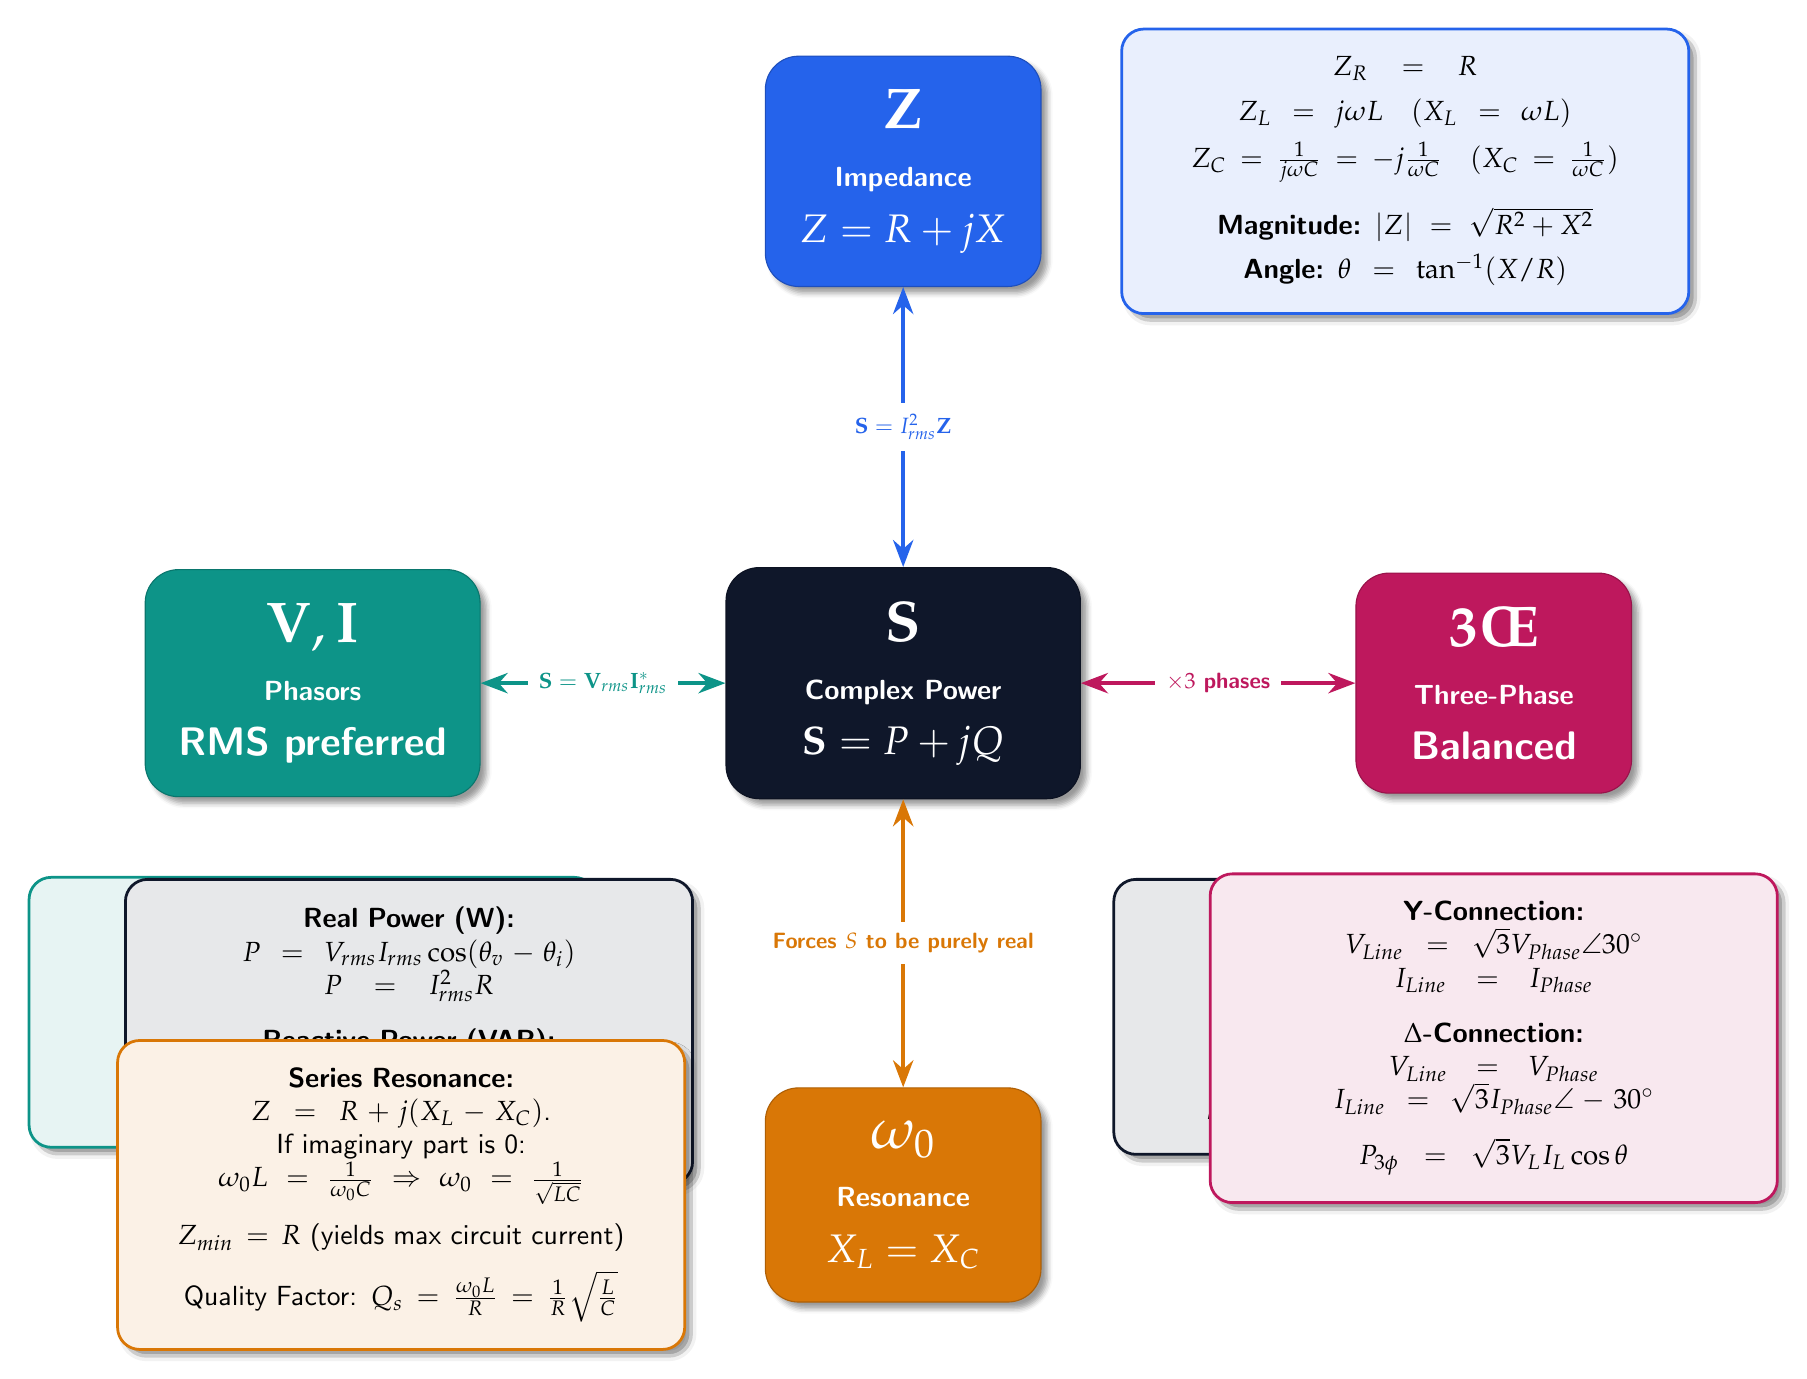
\begin{tikzpicture}[
  hub/.style={rectangle, rounded corners=12pt, draw=#1!80!black, fill=#1, text=white,
    font=\bfseries\sffamily\Large, inner sep=12pt, align=center,
    blur shadow={shadow blur steps=4}, minimum width=3.5cm},
  sat/.style={rectangle, rounded corners=8pt, draw=#1, fill=#1!10,
    font=\sffamily\normalsize, align=center, text width=6.5cm, inner sep=10pt,
    line width=1pt, blur shadow={shadow blur steps=2}},
  rel/.style={<->, >=Stealth, line width=1.5pt, draw=#1},
  lbl/.style={font=\sffamily\footnotesize\bfseries, fill=white, inner sep=4pt, text=#1},
]

%% -- Central Hubs  --------------------------------------------
\node[hub=DeepNavy, minimum width=4.5cm, minimum height=2.2cm] at (0, 0) (S)
  {\huge $\mathbf{S}$\\[3pt]\normalsize Complex Power\\[2pt] $\mathbf{S} = P + jQ$};

\node[hub=ElectricBlue] at (0, 6.5) (Z) {\huge $\mathbf{Z}$\\[3pt]\normalsize Impedance\\[2pt] $Z = R + jX$};
\node[hub=Teal]         at (-7.5, 0) (V) {\huge $\mathbf{V, I}$\\[3pt]\normalsize Phasors\\[2pt] RMS preferred};
\node[hub=Crimson]      at (7.5, 0) (Tri) {\huge $\mathbf{3\phi}$\\[3pt]\normalsize Three-Phase\\[2pt] Balanced};
\node[hub=Amber]        at (0, -6.5) (Res) {\huge $\omega_0$\\[3pt]\normalsize Resonance\\[2pt] $X_L = X_C$};

%% -- Equations (Satellites) --------------------------------------------------
\node[sat=ElectricBlue, right=1.0cm of Z] (bz) {
  $Z_R = R$\\[4pt]
  $Z_L = j\omega L \quad (X_L = \omega L)$\\[4pt]
  $Z_C = \frac{1}{j\omega C} = -j\frac{1}{\omega C} \quad (X_C = \frac{1}{\omega C})$\\[8pt]
  \textbf{Magnitude:} $|Z| = \sqrt{R^2 + X^2}$\\[4pt]
  \textbf{Angle:} $\theta = \tan^{-1}(X/R)$
};

\node[sat=Teal, below=1.0cm of V] (bv) {
  \textbf{Ohm's Law (AC):} $\mathbf{V} = \mathbf{I}Z$\\[6pt]
  $\mathbf{V} = V_{m} \angle \theta_v \quad (\text{Peak})$\\[4pt]
  $\mathbf{V}_{rms} = \frac{V_m}{\sqrt{2}} \angle \theta_v$\\[6pt]
  Timedomain:\\$v(t) = V_m \cos(\omega t + \theta_v)$
};

\node[sat=DeepNavy, below left=1.0cm and 0.4cm of S] (bs1) {
  \textbf{Real Power (W):}\\
  $P = V_{rms} I_{rms} \cos(\theta_v - \theta_i)$\\
  $P = I_{rms}^2 R$\\[8pt]
  \textbf{Reactive Power (VAR):}\\
  $Q = V_{rms} I_{rms} \sin(\theta_v - \theta_i)$\\
  $Q_L > 0$ (Inductor absorbs Q)\\
  $Q_C < 0$ (Capacitor supplies Q)
};

\node[sat=DeepNavy, below right=1.0cm and 0.4cm of S] (bs2) {
  \textbf{Apparent Power (VA):}\\
  $|S| = V_{rms} I_{rms} = \sqrt{P^2+Q^2}$\\[8pt]
  \textbf{Power Factor (pf):}\\
  $pf = \cos(\theta_v-\theta_i) = P/|S|$\\
  \textit{Lagging} = I lags V (Inductive)\\
  \textit{Leading} = I leads V (Capacitive)
};

\node[sat=Crimson, below=1.0cm of Tri] (btri) {
  \textbf{Y-Connection:}\\
  $V_{Line} = \sqrt{3} V_{Phase} \angle 30^\circ$\\
  $I_{Line} = I_{Phase}$\\[8pt]
  \textbf{$\Delta$-Connection:}\\
  $V_{Line} = V_{Phase}$\\
  $I_{Line} = \sqrt{3} I_{Phase} \angle -30^\circ$\\[8pt]
  $P_{3\phi} = \sqrt{3} V_L I_L \cos\theta$
};

\node[sat=Amber, left=1.0cm of Res] (bres) {
  \textbf{Series Resonance:}\\
  $Z = R + j(X_L - X_C)$. If imaginary part is 0:\\
  $\omega_0 L = \frac{1}{\omega_0 C} \Rightarrow \omega_0 = \frac{1}{\sqrt{LC}}$\\[6pt]
  $Z_{min} = R$ (yields max circuit current)\\[6pt]
  Quality Factor: $Q_s = \frac{\omega_0 L}{R} = \frac{1}{R} \sqrt{\frac{L}{C}}$
};

%% Relations
\draw[rel=ElectricBlue] (Z) -- node[lbl=ElectricBlue, midway]{$\mathbf{S} = I_{rms}^2 \mathbf{Z}$} (S);
\draw[rel=Teal] (V) -- node[lbl=Teal, midway]{$\mathbf{S} = \mathbf{V}_{rms}\mathbf{I}_{rms}^*$} (S);
\draw[rel=Crimson] (S) -- node[lbl=Crimson, midway]{$\times 3$ phases} (Tri);
\draw[rel=Amber] (Res) -- node[lbl=Amber, midway]{Forces $S$ to be purely real} (S);

\end{tikzpicture}
\end{center}

\clearpage
%% -----------------------------------------------------------------------------
%% PAGE 5 — OP-AMPS & DIODES (NEW)
%% -----------------------------------------------------------------------------
\cmhead{Indigo}{Op-Amps \& Diodes}{Key Non-Linear Components \& Topologies}

\vspace{10pt}
\begin{center}
\begin{tikzpicture}[node distance=0.8cm and 1.2cm,
  itembox/.style={rectangle, rounded corners=8pt, draw=#1!80!black, fill=#1!5, text width=6.2cm, align=left, font=\sffamily\small, inner sep=10pt, blur shadow={shadow blur steps=2}, line width=1.5pt},
  sectitle/.style={rectangle, rounded corners=8pt, fill=#1, text=white, font=\sffamily\large\bfseries, inner sep=8pt, align=center, blur shadow={shadow blur steps=2}}
]

%% OP AMPS HALF (LEFT)
\node[sectitle=Indigo, text width=13.0cm] at (-7, 7) (Otitle) {\faWaveSquare\enspace Operational Amplifiers};

\node[itembox=Indigo] at (-10.5, 3) (O1) {
  \textbf{\large The Golden Rules} (Ideal Op-Amp)\\[8pt]
  \textbf{1. Infinite Gain ($A \to \infty$)}\\
  Coupled with negative feedback, this forces the inputs to safely approach the same voltage.\\
  $\Rightarrow \mathbf{V_+} = \mathbf{V_-}$ \quad (Virtual Short)\\[8pt]
  \textbf{2. Infinite Input Impedance ($R_{in} \to \infty$)}\\
  No current can enter the input terminals.\\
  $\Rightarrow \mathbf{I_+} = \mathbf{I_-} = \mathbf{0}$\\[8pt]
  \textit{Analysis Strategy:} Always apply KCL at the $V_-$ node. Remember no current goes into the op-amp!
};

\node[itembox=Indigo] at (-3.5, 3) (O2) {
  \textbf{\large Amplifier Foundations}\\[8pt]
  \textbf{Inverting Amplifier}\\[4pt]
  Input connected to $V_-$, $V_+$ grounded.\\
  $\text{KCL: } \frac{V_{in} - 0}{R_{in}} + \frac{V_{out} - 0}{R_f} = 0$\\[4pt]
  $\Rightarrow \mathbf{V_{out} = - \left( \frac{R_f}{R_{in}} \right) V_{in}}$\\[12pt]
  \textbf{Non-Inverting Amplifier}\\[4pt]
  Input connected to $V_+$, $V_-$ feedback grounded.\\
  $\text{KCL: } \frac{V_{out} - V_{in}}{R_f} = \frac{V_{in}}{R_{in}}$\\[4pt]
  $\Rightarrow \mathbf{V_{out} = \left( 1 + \frac{R_f}{R_{in}} \right) V_{in}}$
};

\node[itembox=Indigo] at (-10.5, -3) (O3) {
  \textbf{\large Advanced Topologies}\\[8pt]
  \textbf{Summing Amplifier} (Inverting)\\[4pt]
  Multiple inputs $V_1, V_2, \dots$ to $V_-$.\\
  $V_{out} = - R_f \left( \frac{V_1}{R_1} + \frac{V_2}{R_2} + \dots \right)$\\[12pt]
  \textbf{Difference Amplifier}\\[4pt]
  Takes two inputs and subtracts them.\\
  If $R_1=R_2$ and $R_3=R_4$:\\
  $V_{out} = \frac{R_3}{R_1} (V_2 - V_1)$
};

\node[itembox=Indigo] at (-3.5, -3) (O4) {
  \textbf{\large Dynamic Op-Amps}\\[8pt]
  \textbf{Integrator (Cap in Feedback)}\\[4pt]
  $I_{in} = \frac{V_{in}}{R}$, \quad $I_C = C \frac{d(V_{out}-0)}{dt}$\\
  $V_{out}(t) = -\frac{1}{RC} \int V_{in}(t) dt$\\[12pt]
  \textbf{Differentiator (Cap at Input)}\\[4pt]
  $I_{in} = C \frac{dV_{in}}{dt}$, \quad $I_R = \frac{V_{out}}{R}$\\
  $V_{out}(t) = -RC \frac{dV_{in}}{dt}$
};


%% DIODES HALF (RIGHT)
\draw[SlateGray!40, dashed, line width=2pt] (0, 7.5) -- (0, -6.5);

\node[sectitle=Amber, text width=13.0cm] at (7, 7) (Dtitle) {\faPlay\enspace Diode Models \& Circuits};

\node[itembox=Amber] at (3.5, 3) (D1) {
  \textbf{\large Ideal Diode Model}\\[8pt]
  Acts as a perfect electronic switch.\\[6pt]
  \textbf{ON (Forward Bias):}\\
  Acts as a short circuit (wire). $V_D = 0V$.\\
  Current $I_D \ge 0$ flows freely from P to N.\\[8pt]
  \textbf{OFF (Reverse Bias):}\\
  Acts as an open circuit (break). $I_D = 0A$.\\
  Voltage $V_D < 0$ is blocked.\\[8pt]
  \textit{Analysis rule:} Guess a state (ON/OFF), solve the linear circuit, then verify your guess logic!
};

\node[itembox=Amber] at (10.5, 3) (D2) {
  \textbf{\large Constant Voltage Drop (CVD)}\\[8pt]
  Real diodes require a turn-on voltage (often Silicon = 0.7V).\\[6pt]
  \textbf{ON (Forward Bias):}\\
  Modeled as a battery: $V_D = 0.7V$.\\
  Circuit must provide enough potential to overcome this $0.7V$ threshold. Current leaves positive terminal.\\[8pt]
  \textbf{OFF (Reverse Bias):}\\
  $I_D = 0A$.\\
  Circuit potential is insufficient: $V_D < 0.7V$.
};

\node[itembox=Amber, text width=13.2cm] at (7, -3) (D3) {
  \textbf{\large Zener Regulators (Voltage Anchoring)}\\[8pt]
  Zener diodes operate in the reverse breakdown region to regulate voltage.\\[8pt]
  \textbf{1. Test State:} Remove Zener completely, calculate $V_{load}$ (open circuit voltage across terminals).\\[6pt]
  \textbf{2. Check Breakdown Condition:}\\
  If $V_{load} \ge V_Z$, the Zener is \textbf{ON} and regulating.\\
  It solidly locks the Load Voltage to exactly $V_Z$.\\
  $I_{source} = \frac{V_{source} - V_Z}{R_{series}} \quad , \quad I_{load} = \frac{V_Z}{R_{load}}$\quad, \quad $I_{Zener} = I_{source} - I_{load}$\\[6pt]
  If $V_{load} < V_Z$, the Zener is \textbf{OFF}.\\
  It acts as an open circuit. Load Voltage is exactly the original $V_{load}$.
};

\end{tikzpicture}
\end{center}

\end{document}
